\documentclass[10pt]{beamer}
\usepackage{inputenc}
\usepackage{graphicx}
\usepackage{enumerate}
\usepackage{listings}
\usepackage{caption, subcaption}
\captionsetup[subfigure]{justification=centering}
\captionsetup{font=scriptsize,labelfont=scriptsize}
\usepackage{amsmath}
\usepackage{amssymb}
\usepackage{amsthm}
\usetheme{metropolis}    
\usepackage{verbatim}
\usepackage{alltt}
\usepackage{xcolor}
\usepackage{appendixnumberbeamer}
\usepackage{animate}
\usepackage{xmpmulti}
\usepackage{threeparttable, longtable}
\usepackage{booktabs}
\usepackage{setspace}
\usepackage{adjustbox}
\usepackage[T1]{fontenc}
\usepackage[colorlinks=true, allcolors=blue]{hyperref}
\usepackage{color,soul}
\usepackage{tikz}
\usepackage{multirow}
\usepackage{float}
\usepackage{placeins}

\usepackage{tikz}
\usetikzlibrary{tikzmark,overlay-beamer-styles, calc}

\def\signed #1{{\leavevmode\unskip\nobreak\hfil\penalty50\hskip1em
		\hbox{}\nobreak\hfill #1%
		\parfillskip=0pt \finalhyphendemerits=0 \endgraf}}

\newsavebox\mybox
\newenvironment{aquote}[1]
{\savebox\mybox{#1}\begin{quote}\openautoquote\hspace*{-.7ex}}
	{\unskip\closeautoquote\vspace*{1mm}\signed{\usebox\mybox}\end{quote}}
\newcommand{\backupbegin}{
	\newcounter{finalframe}
	\setcounter{finalframe}{\value{framenumber}}
}
\newcommand{\backupend}{
	\setcounter{framenumber}{\value{finalframe}}
}
\usepackage[normalem]{ulem}
\useunder{\uline}{\ul}{}
\makeatletter
\setbeamertemplate{footline}
{
	\leavevmode%
	\hbox{%
		\begin{beamercolorbox}[wd=.15\paperwidth,ht=2.25ex,dp=1ex,center]{institute in head/foot}%
			\usebeamerfont{title in head/foot}%
			%  \insertshortauthor 
		\end{beamercolorbox}%
		\begin{beamercolorbox}[wd=.6\paperwidth,ht=2.25ex,dp=1ex,center]{institute in head/foot}%
			\usebeamerfont{title in head/foot}%
			\insertshorttitle
		\end{beamercolorbox}%
		\begin{beamercolorbox}[wd=.15\paperwidth,ht=2.25ex,dp=1ex,center]{institute in head/foot}%
			\usebeamerfont{title in head/foot}%
			\insertshortdate
		\end{beamercolorbox}%
		\begin{beamercolorbox}[wd=.1\paperwidth,ht=2.25ex,dp=1ex,right]{institute in head/foot}%
			\usebeamerfont{title in head/foot} 
			\insertframenumber{} / \inserttotalframenumber\hspace*{2ex} 
	\end{beamercolorbox}}%
}

\definecolor{blueucl}{RGB}{0,87,156} 
\setbeamercolor{itemize item}{fg = blueucl}
\setbeamercolor{itemize subitem}{fg = blueucl}
\setbeamercolor{enumerate item}{fg = blueucl}
\setbeamercolor{enumerate subitem}{fg = blueucl}
\setbeamertemplate{itemize item}[triangle]
\setbeamercolor{progress bar}{fg=blueucl}
\setbeamercolor{alerted text}{fg = blueucl}

\lstset{numbers=left, numberstyle=\tiny, stepnumber=1,firstnumber=1,
	numbersep=5pt,
	stringstyle=\ttfamily,
	basicstyle=\footnotesize, 
	showstringspaces=false, 
	stringstyle=\color{blueucl}, 
	tabsize=1
}
\makeatother
\setbeamertemplate{caption}[numbered]
\newcommand{\ep}{\varepsilon}
\newtheorem{assumption}{Assumption}
\newtheorem{proposition}{Proposition}

\title[FlowTrading]{Flow Trading Format: A Laboratory Test}
\author[DF-YL-KL]{Dan Friedman, Yilin Li, Kristian L\'opez Vargas}
\institute[Essex, UCSC]{University of Essex and 
University of California, Santa Cruz}  
\date[4/11/2024]{\textbf{Smith Institute Seminar, Chapman University} \\
April 11, 2024}

\begin{document}
\maketitle

\tableofcontents

\section{Motivation}
\begin{frame}{
The continuous double auction (CDA) market format}
\begin{itemize}
\item dominated in 20th century financial markets 
\item but is now problematic.  %\pause
\end{itemize}
Problems arise from
\begin{itemize}
\item strict price/time priority and 
\item a coarse price grid, 
\item together with modern telecommunications and software.
\end{itemize} %\pause
The result is HFT: huge investment to acquire millisecond (or even microsecond) advantage to snap up stale bids/asks, causing
%\pause
\begin{itemize}
\item unequal access: ``tilted playing field''
\item 10's or 100's of \$billions in unproductive rent-seeking, %\pause
\item reduced true liquidity due to toxic takers %\pause
\item increased danger of ``flash crashes,'' as unknowable algorithms interact.
   \end{itemize}
\end{frame}

\begin{frame}{Reform proposals}
for 21st century financial market formats include
    \begin{itemize}
\item IEX: see e.g., M. Lewis (2014), Aldrich and Friedman (2023); %\pause
\item FBA: see e.g., Budish et al (2015), Aldrich and Lopez (2022); and %\pause
\item Flow markets:  Kyle \& Lee (2017), Budish et al. (2023).
\end{itemize}
The last is my personal favorite, and the subject of today's presentation.
\end{frame}

\begin{frame}{Claimed Benefits of Flow markets.}
Its proponents argue that Flow markets provide a
\begin{enumerate}
 \item natural solution to HFT problems, and a %\pause
\item natural way to minimize price impact. 
\begin{itemize}
    \item CDA provokes arms race to shred orders. 
\end{itemize} %\pause
\item The format also facilitates combinatorial trade for inter-related assets (`package trades').
\end{enumerate} 
\end{frame}

\begin{frame}{Our project}
compares CDA and Flow market formats in a simple lab environment. %\pause

Comparison criteria include measures of
\begin{itemize}
 \item  price stability and efficiency; %\pause
\item trading volume, pace and churn; and %\pause
\item buyer vs seller profits and overall efficiency. 
\end{itemize} 
Sets stage for (but does not yet include) investigation of  package bidding, nor HFT distortions.
\end{frame}

% \begin{frame}{Motivation}
%     \begin{itemize}
%         \item Exchanges based in CDA exhibit several important \textbf{flaws}.
%         \item \textbf{CDA} forces \textbf{discreteness} in price and quantity (demand and supply curves are discontinuous step functions). 
%     \end{itemize}
%     \textbf{Problem 1: Price Impact} 
%     \begin{itemize}
%         \item CDA only allows agents to submit intentions to \textbf{trade at once} (e.g. BUY, 100 Shares, at \$20)
%         \item Theory and vast evidence show that if processing/sending orders is cheap, traders' optimal strategy is to \textbf{shred} orders not to have a \textbf{price impact} (send many orders with small quantities to obtain a good average price)
%         \item Since the \textbf{access} to computation and communication technology is \textbf{heretogeneous}, CDA effectively favors a subset of agents
%         \item The flow format moves the implementation of \textbf{shredding into the exchange}, leveling the field
%     \end{itemize}
% \end{frame}

% \begin{frame}{Motivation}
%     \textbf{Problem 2: Picking Off} 
%     \begin{itemize}
%         \item The CDA rewards traders with high speed and short-term information. How?
%         \item Excess demand or supply occur often at the trading price, making the rationing rule relevant. The rule is usually based on time priority, creating a comm-tech arms race among traders
%         \item The outcome is a massive cooperation dilemma % BCS: better off without investing in comm-tech
%         \item Who is to blame? The HFTs or the CDA built-in design flaws?
%         \item We think a design fix is better than heavy handed solutions (\textbf{FLOW}, IEX, FBA, etc)
%         \item Which design is better? \textbf{Observational data} is insufficient to resolve the question. \textbf{Experimentation} is necessary. 
%     \end{itemize}
% \end{frame}

% \begin{frame}{Related Literature}
%     \begin{itemize}
%     % \item What is the optimal trading strategy when there is \textbf{price impact}?
%     %\item Vayanos (1999) and Du and Zhou (2017) show that agents prefer to \textbf{smooth trade} across rounds to limit price impact when information about endowments is private.
    
%     \item Vayanos (1999), Du and Zhou (2017) show that \textbf{smooth trading} is equilibrium behavior when information about endowments is private. 
%     % Obiz (2017) present a similar result in a continuous-time model with many competitors. % vayanos1999strategic

%     \item Kyle \& Lee (2017) and Budish et al (2015) highlight the design problem and both propose a design change. KL17 propose the ``flow'' design; and BCS15 propose the frequent batch auction (FBA). % kyle2017toward; budish2015highfrequency

%     \item Aldrich and Friedman (2022) theoretically study the IEX format (speed bumps and pegged orders). % aldrich2022order

%     %  \item In contrast, Rostek et al. (2015) argue that allowing for higher trading frequency increases welfare in symmetric information markets. 

%     \item Budish et al (2020) discusses the existing \textbf{lack of incentives to adopt new market designs} that reduce latency arbitrage and deactivates the high-frequency trading arms race. % budish2020theory

%     \item Budish et al (2022) extend the flow trading design to multiple assets. % budish2022flow

%     % \item Vayanos (1999): When information about endowments is private (and independent), smooth trading constitutes an equilibrium in a multiple-round setting. Du and Zhou (2017) predicts the same outcome in a similar setting. 
%     % \item In a continuous-time model, Kyle et al. Obiz (2017) show that agents trade gradually to limit price impact.
%     % \item Biais, Foucault, and Moinas (2013) shows that the ability to privately acquire information leads to an overinvestment in speed. 

%     %where strategics agents receive random stock endowments ( private info) and trade to share dividend risk 
%     %\item Du and Zhou (2017)
%     %\item Biais, Foucault, and Moinas (2013) \item Dynamic Thin Markets (2015):

% \end{itemize}
% \end{frame}


% \begin{frame}{Related Literature}
%     \begin{itemize}
%         \item  Biais, Foucault, and Moinas (2015) show that the ability to privately acquire information leads to an \textbf{over-investment in communication speed}. % biais2015equilibrium
%         %$\rightarrow$ Net welfare gains from removing speed-related rents. 
    
    
%         % This occurs when exchange trading fees are competitive but exchages can earn profits from the sale of speed technology -> little incentives for socially optimal market design.
%         \item Many studies have compared CDA to other formats under different settings (e.g., Friedman, 1996 \& 1999)
    
%         \item Aldrich \& Lopez Vargas (2020) compare CDA with Frequent-Batch Auctions (FBA). % aldrich2020experiments

%         %\item Andryl \& Shikilko (2016) find that exogenously reducing available trading speed diminishes adverse selection and, overall, liquidity improves significantly. 

%         % \item Since only CDA is the prefered market design, laboratory settings are required to empirical compare its performance to other formats.
    
%         \item ...
%     \end{itemize}
% \end{frame}

\section{Market Formats}
\begin{frame}{Continuous Double Auction (CDA) Format}
processes standard limit orders.
\begin{itemize}
    \item These orders are defined by \textbf{three parameters}:$\rightarrow$ ``\underline{Buy/sell} up to \underline{$Q_{max}$} (shares) at a price of \underline{$P$} (dollars per share) or better."
\item Asynchronous order submission within a known time interval. 
\begin{itemize}
\item If a new order does not \textbf{cross} a queued contra-side order, then it is queued in the book. 
\item If it does cross, then it transacts immediately at the best price(s) on the other side of the market.
\end{itemize}
\item Strict \textbf{(price, time) priority}. If there is a tie on price, then older orders are filled first.
    \end{itemize} 
\end{frame}

% \begin{frame}{Market Format 1: The Continuous Double Auction (CDA)}
%     For a \textbf{buy order} placed at time $t_0$, let $Q_{(t_{0},t)}$ denote the cumulative \textbf{quantity executed} in interval $[t_0, t ]$ for $t > t_{0}$:
%     \begin{align}
%     Q_{(t_{0},t)}=
%     \begin{cases}
%     Q_{max} & \text{ if } p_{min(t_{0},t)} < P \\
%     \alpha(t_{0},t)Q_{max} & \text{ if } p_{min(t_{0},t)} = P  \\
%     0  & \text{ if } p_{min(t_{0},t)} > P \\
%     \end{cases}
%     \end{align}
%     where $\alpha(t_{0},t)\in [0,1]$ depends on the rationing rule and $p_{\min}(t_0,t)$ is defined as the minimum price $p(t)$ during the interval $t \in [t_0,t]$. \\
%     \vspace{1cm}
%     It is similar for the individual supply curve. It is a non-decreasing step function.
% \end{frame}

% \begin{frame}{Market Format 1: The CDA - Example - Individual}
%     \begin{figure}
%         \centering
%         \includegraphics[width=\textwidth]{production/contract/production_1.png}
%         \caption{Standard Limit Orders}
%         \label{fig:cda}
%     \end{figure}
% \end{frame}

\begin{frame}{CDA Example Market}
    \begin{figure}[H]
        \centering
        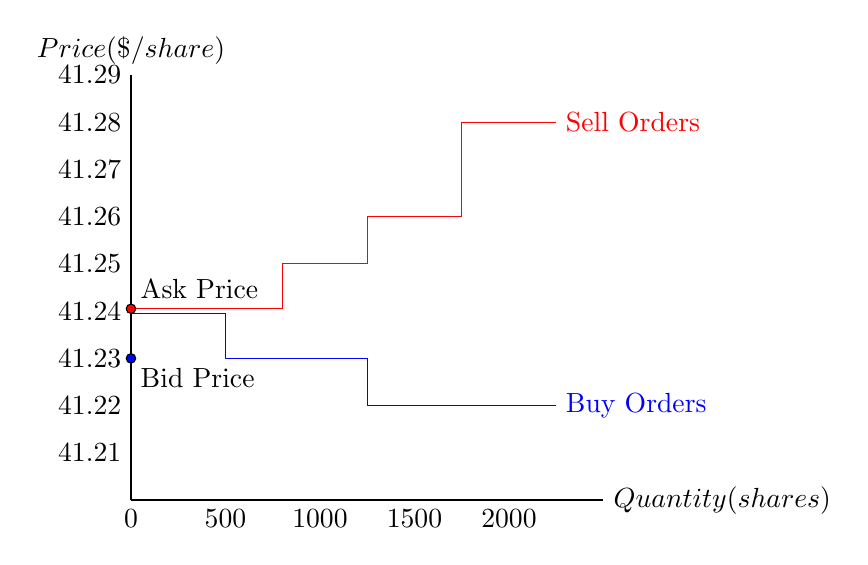
\begin{tikzpicture}[scale=.6]
        \draw[thick,-] (0,0) -- (0,9) node[above]{$Price (\$/share)$};
        \draw[thick,-] (0,0)--(10,0) node[right]{$Quantity (shares)$};
        \node[left] at (0,1) {$41.21$};
        \node[left] at (0,2) {$41.22$};
        \node[left] at (0,3) {$41.23$};
        \node[left] at (0,4) {$41.24$};
        \node[left] at (0,5) {$41.25$};
        \node[left] at (0,6) {$41.26$};
        \node[left] at (0,7) {$41.27$};
        \node[left] at (0,8) {$41.28$};
        \node[left] at (0,9) {$41.29$};
        \node[below] at (2,0) {$500$};
        \node[below] at (4,0) {$1000$};
        \node[below] at (6,0) {$1500$};
        \node[below] at (8,0) {$2000$};
        \node[below] at (0,0) {$0$};
        \draw[blue,solid] (0,3.95) -- (2,3.95) -- (2,3) -- (5,3) -- (5,2) -- (9,2) node[right]{Buy Orders} ;
        \draw[red,solid] (0,4.05) -- (3.2,4.05) -- (3.2,5) -- (5,5) -- (5,6) -- (7,6) -- (7,8) -- (9,8) node[right]{Sell Orders};
        \node[above right] at (0,4.05) {Ask Price};
        \draw[fill=red] (0,4.05) circle [radius=.1];
        \node[below right] at (0,3) {Bid Price};
        \draw[fill=blue] (0,3) circle [radius=.1];
        \end{tikzpicture}
        \caption{Standard Limit Order Book}
    \end{figure}
\end{frame}

\begin{frame}{CDA Timing Issues}
1. Early bird special  
    \begin{itemize}
        \item Since market supply and demand are discontinuous step functions of price, there is \textbf{no guarantee of a single point of intersection}: there can be excess of demand (supply), and often there is. 
        \item Hence, \textbf{an allocation rule} to determine $\alpha(t_0, t)$ is needed (e.g., time priority, or pro-rata)
\item In most existing financial markets, orders are \textbf{prioritized} based on \textbf{the time they arrive}, so high speed is rewarded
\item If an agent can \textbf{react to a relevant signal} (even if public) \textbf{faster} (even if only a tiny bit) than other traders, then she can \textbf{pick off stale orders} from other traders and reverse position after the information has spread in the market.
\item  Thus: tilted playing field, rent-seeking, toxic takers $\implies$ illiquidity, increased flash crash risk.
    \end{itemize}
    2. To avoid adverse price pressure, traders will want to \textbf{shred} large orders.
    \end{frame}

\begin{frame}{Market Format 2: The FLOW}
    \begin{itemize}
\item Continuous scaled limit orders have \textbf{five parameters}: $\rightarrow$ ``\underline{Buy/Sell} up to a cumulative total of  \underline{$Q_{max}$} (shares) at maximum rate \underline{$U_{max}$} (shares per hour) at prices between \underline{$P_{L}$} and \underline{$P_{H}$} (dollars per share)."
\item Consider a buy order. The (buying rate or) flow demand $U(p(t))$ is the decreasing pw linear function:
\begin{align}
                U{(p(t))}=
                \begin{cases}
                    U_{max} & \text{ if } p{(t)} < P_{L} \\
                    (\frac{P_{H}-p(t)}{P_{H}-P_{L}})U_{max} & \text{ if } P_L \leq p{(t)} \leq P_H \\
                    0  & \text{ if } p{(t)} > P_{H} \\
                \end{cases}
\end{align}
        where $p(t)$ is the clearing price at time $t$.
\item The flow supply (rate) is an analogous pw linear monotone \textbf{increasing} function of $p(t)$
    \end{itemize}
\end{frame}

\begin{frame}{Market Format 2: FLOW - Example - Individual}
    \begin{figure}
        \centering
        
\includegraphics[width=\textwidth]{figures/flow.png}
        \caption{Continuous Scaled Limit Orders}
        \label{fig:flow}
    \end{figure}
\end{frame}

\begin{frame}{Market Format 2: FLOW - Example - Market}
    \begin{figure}[H]
        \centering
        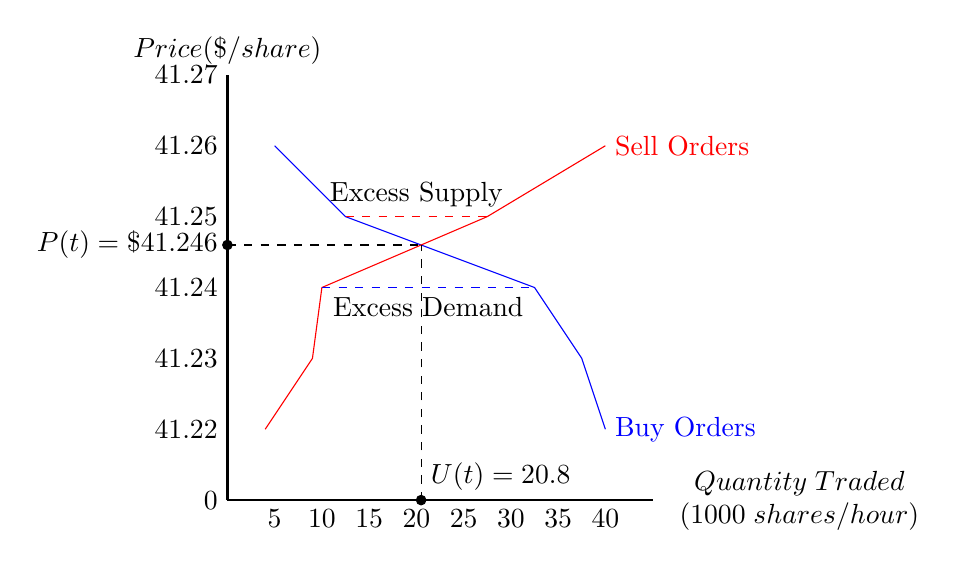
\begin{tikzpicture}[scale=0.6]
            \draw[thick,-] (0,0) -- (0,9) node[above]{$Price (\$/share)$};
            \draw[thick,-] (0,0)--(9,0) node[right]{\begin{tabular}{c}
                 $Quantity \; Traded$ \\
                 $(1000 \; shares/hour)$
            \end{tabular}};
            \node[left] at (0,1.5) {$41.22$};
            \node[left] at (0,3.0) {$41.23$};
            \node[left] at (0,4.5) {$41.24$};
            \node[left] at (0,6.0) {$41.25$};
            \node[left] at (0,7.5) {$41.26$};
            \node[left] at (0,9.0) {$41.27$};
            \node[below] at (1,0) {$5$};
            \node[below] at (2,0) {$10$};
            \node[below] at (3,0) {$15$};
            \node[below] at (4,0) {$20$};
            \node[below] at (5,0) {$25$};
            \node[below] at (6,0) {$30$};
            \node[below] at (7,0) {$35$};
            \node[below] at (8,0) {$40$};
            \node[left] at (0,0) {$0$};
            \draw[blue,solid] (1,7.5) -- (2.5,6.0) -- (6.5,4.5) -- (7.5,3) -- (8,1.5) node[right]{Buy Orders} ;
            \draw[red,solid] (0.8,1.5) -- (1.8,3) -- (2,4.5) -- (5.5,6) -- (8,7.5) node[right]{Sell Orders};
            \draw[red,dashed] (2.5,6.0) -- (5.5,6.0);
            \draw[blue,dashed] (2,4.5) -- (6.5,4.5);
            \node[black,above] at (4,6.0) {Excess Supply};
            \node[black,below] at (4.25,4.5) {Excess Demand};
            \draw[dashed] (4.1,0) -- (4.1,5.4);
            \draw[dashed] (0,5.4) -- (4.1,5.4);
            \node[above right] at (4.1,0) {$U(t)=20.8$};
            \draw[fill] (4.1,0) circle [radius=.1];
            \node[left] at (0,5.4) {$P(t)=\$41.246$};
            \draw[fill] (0,5.4) circle [radius=.1];
        \end{tikzpicture}
        \caption{Continuous Scaled Limit Order Book}
    \end{figure}
\end{frame}

\begin{frame}{Market Format 2: FLOW}
\begin{itemize}
\item Both the downward sloping demand schedule and upward sloping supply schedule are \textbf{piece-wise linear} functions of price $\rightarrow$ \textbf{unique} price and rate of shares per hour. %\pause
\item All continuous scaled limit orders ares treated \textbf{symmetrically} and executed \textbf{simultaneously} at the market clearing price %\pause
        \item \textbf{opportunities} to do order \textbf{shredding} are now \textbf{distributed equally} across agents, as now instructions to shred are ``moved into the exchange" %\pause
        \item Consequently, now the
        \textbf{fastest trader} or the ones that can send massive number of messages to update orders are not rewarded
    \end{itemize}
\end{frame}

\section{Lab Procedures}

\begin{frame}{Experiment Design: Main Elements}
    \begin{itemize}
        \item Groups of 8 traders will participate in an asset market for 22 trading periods, each lasting two minutes (2 practice + 20 payment)
        \item \textbf{Incentives to trade}: In each trading period, the computer provides a buy or sell contract committing to buy or sell up to $x$ shares at some point during the trading period (e.g., Computer will buy up to 300 shares from you at price 13 ECU at second 115) 
        \item Contracts are private information %\pause
        \item Subjects' inventories are restricted to be $[-Q_{contract}, 0]$ for those with a sell contract or $[0, Q_{contract}]$ for those with a buy contract
        \item \textbf{Choice Space}: Subjects can submit or update buy and/or sell orders %\pause
        \item \textbf{Treatments}: \{CDA, FLOW\} (between-group)
        \item Three sets of contacts varied across 5 blocks of 4 periods each. 
    \end{itemize}
\end{frame}

\begin{frame}{Experiment Design: Contracts}
    
\begin{figure}
    \centering
    % \caption{Contract Configurations}
    \begin{subfigure}[c]{0.33\linewidth}
        \centering
            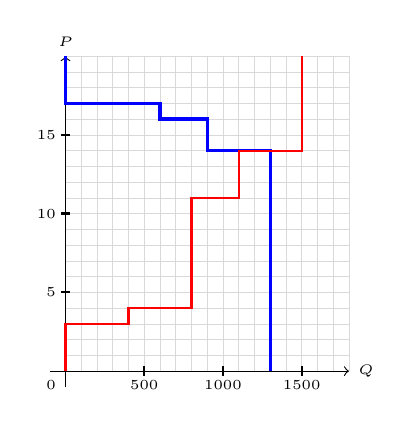
\begin{tikzpicture}[scale=.2]
                % create grid
                \draw[help lines, gray!30] (0,0) grid (18,20);
                
                % Draw axes
                \draw[->] (-1,0) -- (18,0) node[font=\tiny,right] {$Q$};
                \draw[->] (0,-1) -- (0,20) node[font=\tiny,above] {$P$};
              
                % Draw step functions
                \draw[blue, very thick] (0,20) -- (0,17) -- (6,17) -- (6,16) -- (9,16) -- (9,14) - - (13,14) -- (13,0) ;
                \draw[red, thick] (0,0) -- (0,3) -- (4,3) -- (4,4) -- (8,4) -- (8,11) --  (11,11) -- (11,14) -- (15,14) -- (15,20);
                
                % % Add labels
                \node[font=\tiny,below left] at (0,0) {$0$};
                \foreach \x in {5,10,15} {
                  \node[font=\tiny,below] at (\x,0) {$\x00$};
                }
                \foreach \y in {5,10,15} {
                  \node[font=\tiny,left] at (0,\y) {$\y$};
                }
                
                % % Add thicker ticks (Q)
                \draw[black, thick] (5,-0.3) -- (5,0.3);
                \draw[black, thick] (10,-0.3) -- (10,0.3);
                \draw[black, thick] (15,-0.3) -- (15,0.3);

                % % Add thicker ticks (P)
                \draw[black, thick] (-0.3,5) -- (0.3,5);
                \draw[black, thick] (-0.3,10) -- (0.3,10);
                \draw[black, thick] (-0.3,15) -- (0.3,15);
            \end{tikzpicture}
        \subcaption{\tiny Block 1 (T1-T4) \\ and Block 5 (T17-T20)}
    \end{subfigure}%
    \begin{subfigure}[c]{0.33\linewidth}
        \centering
        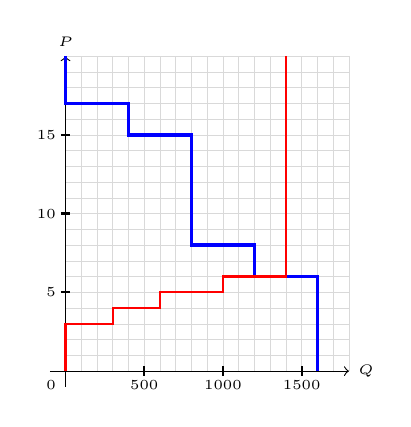
\begin{tikzpicture}[scale=.2]
            % create grid
            \draw[help lines, gray!30] (0,0) grid (18,20);
            
            % Draw axes
            \draw[->] (-1,0) -- (18,0) node[font=\tiny,right] {$Q$};
            \draw[->] (0,-1) -- (0,20) node[font=\tiny,above] {$P$};
          
            % Draw step functions
            \draw[blue, very thick] (0,20) -- (0,17) -- (4,17) -- (4,15) -- (8,15) -- (8,8) -- (12,8) -- (12,6) -- (16,6) -- (16,0);
            \draw[red, thick] (0,0) -- (0,3) -- (3,3) -- (3,4) -- (6,4) -- (6,5) -- (10,5) -- (10,6) -- (14,6) -- (14,20);
            
            % % Add labels
            \node[font=\tiny,below left] at (0,0) {$0$};
            \foreach \x in {5,10,15} {
              \node[font=\tiny,below] at (\x,0) {$\x00$};
            }
            \foreach \y in {5,10,15} {
              \node[font=\tiny,left] at (0,\y) {$\y$};
            }

            % % Add thicker ticks (Q)
            \draw[black, thick] (5,-0.3) -- (5,0.3);
            \draw[black, thick] (10,-0.3) -- (10,0.3);
            \draw[black, thick] (15,-0.3) -- (15,0.3);

            % % Add thicker ticks (P)
            \draw[black, thick] (-0.3,5) -- (0.3,5);
            \draw[black, thick] (-0.3,10) -- (0.3,10);
            \draw[black, thick] (-0.3,15) -- (0.3,15);
        \end{tikzpicture}
        \subcaption{\tiny Block 2 (T5-T8) \\ and Block 4 (T13-T16)}
    \end{subfigure}%
    \begin{subfigure}[c]{0.33\linewidth}
        \centering
        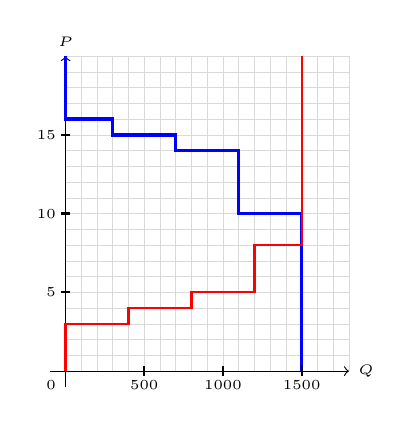
\begin{tikzpicture}[scale=.2]
            % create grid
            \draw[help lines, gray!30] (0,0) grid (18,20);
            
            % Draw axes
            \draw[->] (-1,0) -- (18,0) node[font=\tiny,right] {$Q$};
            \draw[->] (0,-1) -- (0,20) node[font=\tiny,above] {$P$};
          
            % Draw step functions
            \draw[blue, very thick] (0,20) -- (0,16) -- (3,16) -- (3,15) -- (7,15) -- (7,14) -- (11,14) -- (11,10) -- (15,10) -- (15,0);
            \draw[red, thick] (0,0) -- (0,3) -- (4,3) -- (4,4) -- (8,4) -- (8,5) -- (12,5) -- (12,8) -- (15,8) -- (15,20);
            
            % % Add labels
            \node[font=\tiny,below left] at (0,0) {$0$};
            \foreach \x in {5,10,15} {
              \node[font=\tiny,below] at (\x,0) {$\x00$};
            }
            \foreach \y in {5,10,15} {
              \node[font=\tiny,left] at (0,\y) {$\y$};
            }

            % % Add thicker ticks (Q)
            \draw[black, thick] (5,-0.3) -- (5,0.3);
            \draw[black, thick] (10,-0.3) -- (10,0.3);
            \draw[black, thick] (15,-0.3) -- (15,0.3);

            % % Add thicker ticks (P)
            \draw[black, thick] (-0.3,5) -- (0.3,5);
            \draw[black, thick] (-0.3,10) -- (0.3,10);
            \draw[black, thick] (-0.3,15) -- (0.3,15);
        \end{tikzpicture}
        \subcaption{\tiny Block 3 (T9 - T12)}
    \end{subfigure}
    \caption{\textbf{Contract configurations across trading blocks.}  \footnotesize
Vertical axis is price (ECU per share) and horizontal axis is quantity (shares). Each panel plots the step‐function demand schedule (thick blue) and supply schedule (red).  
The intersection of the two schedules determines the competitive‐equilibrium price–quantity pair for that block.  
Panel (a) applies to Blocks 1 (T1–T4) and 5 (T17–T20) of experiment; panel (b) to Blocks 2 (T5–T8) and 4 (T13–T16); panel (c) to Block 3 (T9–T12). }
% \label{fig:contract-configs}
    \label{fig:3contract_configs_new}
\end{figure}

\end{frame}


\begin{frame}{Experiment Design: Interface - FLOW Animation}
  \animategraphics[loop,controls,width=\linewidth]{10}{figures/flow_animation/flow_animation-}{0}{419}
\end{frame}


\begin{frame}{Experiment Design: Interface - FLOW}
    \begin{figure}[H]
        \centering
        
\includegraphics[width=\textwidth]{figures/flow_ui.png}
        \caption{FLOW UI}
        \label{fig:flow_ui}
    \end{figure}
\end{frame}


\begin{frame}{Experiment Design: Interface - CDA}
    \begin{figure}[H]
        \centering
        
\includegraphics[width=\textwidth]{figures/cda_ui.png}
        \caption{CDA UI}
        \label{fig:cda_ui}
    \end{figure}
\end{frame}

\begin{frame}{Experiment Design: Interface - CDA Animation}
  \animategraphics[loop,controls,width=\linewidth]{10}{figures/cda_animation/cda_animation-}{0}{252}
\end{frame}




\begin{frame}{Experiment Design: Procedures}
    \begin{itemize}
        \item We paid the cumulative profits of all 20 payment periods
        \item Exchange rate is 1000 ECUs = 1 USD and show-up fee is 7 USD %\pause
        \item Experiment software was designed and developed at UCSC's LEEPS Laboratory
        \item Experiment sessions were conducted in person at LEEPS Laboratory
        \item So far have 5  FLOW and 5 CDA sessions
    \end{itemize}
\end{frame}

\subsection{Outcomes and Hypotheses}
\begin{frame}{Outcomes}
    \begin{itemize}
        \item For \textbf{trading behavior}, we study: 
     the number of orders, the size of the orders, submitted prices, and
     the maximum execution rate in Flow market. %\pause
        \item For \textbf{market performance}, we study:
        \begin{itemize}
        \item \textit{Absolute Price Change}, $|P_t - P_{t-1}|$. 
        \item \textit{Price volatility}, $(\ln P_t - \ln P_{t-1})$ 
         \item \textit{Trading Volume}, $Q$ (at the market-period level)
\item\textit{Informational [in]Efficiency},  \( |P_t - P_{\text{CE}}| \). 
    \item\textit{Allocative Efficiency}, measured as \( \Pi/\Pi_{\text{CE}}\) (at the market-period level). 
        \end{itemize}
     
    \end{itemize}
\end{frame}

\begin{frame}{Hypotheses}
    \begin{itemize}
        \item[H1] \textit{Traders will fragment orders more
(i.e., submit a larger number of smaller quantity orders) in CDA format than in Flow format.} %\pause
\vspace{0.3cm}
        \item[H2] \textit{Price volatility will be lower with the Flow format than with the CDA.}%\pause
\vspace{0.3cm}        
        \item[H3] \textit{(a) Trading volume with CDA and Flow formats will be similar. \\ (b) Both will move within each trading block towards the minimum volume that sustains competitive equilibrium.} %\pause
\vspace{0.3cm}        
        \item[H4] \textit{The CDA and Flow formats will exhibit similar levels of (a) informational and (b) allocative efficiency.} %\pause
    \end{itemize}
\end{frame}


\section{Results}

\begin{frame}{Descriptive Stats: Traders' Behavior}
\begin{table}[H]
    \centering
    % \caption{Summary Statistics: Traders' Behavior}
    \resizebox{.95\textwidth}{!}{
    \begin{tabular}{lcccccc}
    \toprule
    ~                               & \multicolumn{2}{c}{T1 - T20} & \multicolumn{2}{c}{T1 - T10}  & \multicolumn{2}{c}{T11 - T20} \\
                                    & CDA       & FLOW      & CDA       & FLOW      & CDA       & FLOW      \\
    \midrule ↩
    % \multicolumn{7}{l}{\textbf{(a) Trader Behavior}} \\
    % \hline \\[-1.8ex]
     Number of Orders                       & 32       & 24            & 31       & 25            & 32        & 23            \\
     \hspace{3mm}Seller             & 17       & 12            & 17       & 13            & 17        & 11            \\
     \hspace{3mm}Buyer              & 15       & 12            & 15       & 12            & 15        & 12            \\
     % Order Size                     & 42       & 72            & 44       & 63            & 40        & 80            \\
     \\
     Quant. per Order                 & 113      & 182           & 115      & 180           & 111       & 185           \\
     \hspace{3mm}Seller             & 115      & 185           & 118      & 184           & 111       & 185           \\
     \hspace{3mm}Buyer              & 114      & 188           & 116      & 184           & 113       & 191           \\
     \\
     Order Price                    & 8.93     & [6.78, 12.64] & 9.18     & [7.15, 13.01] & 8.68      & [6.41, 12.28] \\
     \hspace{3mm}Seller             & 10.7     & [9.21, 15.46] & 11.13    & [9.76, 16.04] & 10.27     & [8.66, 14.88] \\
     \hspace{3mm}Buyer              & 6.9      & [4.22, 9.71]  & 7.01     & [4.26, 9.71]  & 6.79      & [4.19, 9.71]  \\

    \\
     Order Max Rate                 &           & 19.62         &           & 17.78         &           & 21.46         \\
     \hspace{3mm}Seller             &           & 19.67         &           & 18.06         &           & 21.29         \\
     \hspace{3mm}Buyer              &           & 20.15         &           & 17.93         &           & 22.37         \\
    \bottomrule
    \end{tabular}}
    \label{tab:summary_stat_trader}
\end{table}
    
\end{frame}

\begin{frame}{Descriptive Stats: Market Performance}
    
    \begin{table}
    \centering
    % \caption{Summary Statistics: Market Performance}
    % \renewcommand{\arraystretch}{1.1}
     \resizebox{\textheight}{!}{
    \begin{threeparttable}
    \begin{tabular}{lcccccc}
    \toprule
    
    ~                               & \multicolumn{2}{c}{T1 - T20} & \multicolumn{2}{c}{T1 - T10}  & \multicolumn{2}{c}{T11 - T20} \\
                                    & CDA       & FLOW      & CDA       & FLOW      & CDA       & FLOW      \\
    \midrule 
     \\[-1.8ex] 
      \multicolumn{7}{l}{\textit{\textbf{(a)} Price Statistics} (Avg. Equil Price = $9.8$ ECUs)} \\
    % \hline 
     \\[-1.8ex]    
     Clearing Prices ($P_t$, ECUs)              & 8.62      & 9.37      & 9.04      & 9.57      & 8.21      & 9.18      \\
     \hspace{3mm}(Std. Dev.)                    & (2.77)    & (2.54)    & (2.95)    & (2.75)    & (2.51)    & (2.29)    \\
     $ \lvert  P_{t}-P_{t - 1} \rvert $         & 0.57      & 0.39      & 0.58      & 0.39      & 0.55      & 0.4       \\
     Std. Dev. of $(\ln P_{t} - \ln P_{t - 1})$ & 0.14      & 0.07      & 0.15      & 0.07      & 0.13      & 0.07     \\    
     \\ [-1.8ex]
     \multicolumn{7}{l}{\textit{\textbf{(b)} Volume, Transaction Intensity}} \\
     \\ [-1.8ex]
     Traded Volume (shares)                     & 1138      & 959       & 1097      & 872       & 1179      & 1046      \\
     Traded Vol. / $Q_{\text{CE}}$. (\%)        & 93.6      & 78.8      & 90.3      & 71.1      & 96.9      & 86.4      \\
     Filled Contract / $Q_{\text{CE}}$ (\%)     & 85.2      & 77.1      & 81.0      & 69.8      & 89.3      & 84.5      \\
     Num. of Trans.                             & 14        &           & 13        &           & 15        &           \\
     Mean Transaction Size                      & 78        &           & 82        &           & 74        &           \\
     \hspace{3mm}(Std. Dev.)             & (61)      &           & (61)      &           & (60)      &           \\
     Clearing Rate ($q/sec$)                 &           & 9.37      &           & 9.54      &           & 9.2       \\
     \hspace{3mm}(Std. Dev.)             &           & (2.6)     &           & (2.8)     &           & (2.4)     \\
     \\ [-1.8ex]
     \multicolumn{7}{l}{\textit{\textbf{(c)} Efficiency and Buyer-Seller Inequality}} \\
     \\ [-1.8ex]
     Info. Effic.: $\lvert P_t - P_{\text{CE}} \rvert $        & 2.16      & 2.08      & 2.19      & 2.32      & 2.14      & 1.84      \\     
     Alloc. Effic.: $\Pi$ / $\Pi_{\text{CE}}$ ($\times 100$)          & 84.3      & 81.81     & 79.76     & 77.31     & 88.85     & 86.31     \\
     
     ${\Pi^{\text{buy}}}/{\Pi^{\text{buy}}_{\text{CE}}} - {\Pi^{\text{sell}}}/{\Pi^{\text{sell}}_{\text{CE}}}$ 
     ($\times 100$) & 53.7      & 11.18     & 27.38     & -5.16     & 80.03     & 27.51     \\
     \\[-1.8ex] 
    \bottomrule 
    \end{tabular}
    \begin{tablenotes}[para,flushleft]
      \footnotesize
    \end{tablenotes}
    \end{threeparttable}
   }
    \label{tab:summary_stat}
\end{table}
\end{frame}


\begin{frame}{Descriptive: Transaction Price Dynamics}
    \begin{figure}[H]
        \centering
        \begin{subfigure}[b]{0.85\textwidth}
            \centering
            
\includegraphics[width=1.15\linewidth]{figures/Grp-CDA-priceTrim.pdf}
            %\caption{CDA}
            \label{price_flow}
        \end{subfigure}
        \begin{subfigure}[b]{0.85\textwidth}
            \centering
            
\includegraphics[width=1.15\linewidth]{figures/Grp-Flow-priceTrim.pdf}
           % \caption{FLOW}
            \label{price_cda}
        \end{subfigure}
       % \caption{Clearing Prices}
    \end{figure}
    % \vspace{-15pt}
    % \scriptsize{The vertical dotted lines are period breaks. The first 10 seconds from each trading period are left out. The lighter colors represent individual groups.} 
\end{frame}

\begin{frame}{Descriptive: Volume and Surplus Dynamics}
    \begin{figure}
        \centering
        % First row: Volume Trends
        \begin{subfigure}[b]{0.48\linewidth}
            \centering
            
\includegraphics[width=\linewidth]{figures/groups_cda_quantity.png}
            \caption{CDA - Traded Volume}
            \label{fig:combined_volume_cda}
        \end{subfigure}%
        \hfill % Space between the figures
        \begin{subfigure}[b]{0.48\linewidth}
            \centering
            
\includegraphics[width=\linewidth]{figures/groups_flow_quantity.png}
            \caption{FLOW - Traded Volume}
            \label{fig:combined_volume_flow}
        \end{subfigure}
        
        % Second row: Realized Surplus
        \begin{subfigure}[b]{0.48\linewidth}
            \centering
            
\includegraphics[width=\linewidth]{figures/groups_cda_surplus.png}
            \caption{CDA - Realized Surplus}
            \label{fig:combined_surplus_cda}
        \end{subfigure}%
        \hfill % Space between the figures
        \begin{subfigure}[b]{0.48\linewidth}
            \centering
            
\includegraphics[width=\linewidth]{figures/groups_flow_surplus.png}
            \caption{FLOW - Realized Surplus}
            \label{fig:combined_surplus_flow}
        \end{subfigure}
    \end{figure}
\end{frame}

\begin{frame}{Regression Analysis}
For each metric, we estimate: 
\begin{equation} \label{eq:reg}
    y_{g,t} = \alpha + \sum^{4}_{i = 1} \left(\beta_i \; \text{Block}_i\right) + \gamma \; \text{FLOW}_{g,t} + \theta \; \text{Period}_{g,t} + \epsilon_{g,t}
\end{equation}
where $y_{g,t}$ is an outcome  indexed by group (i.e., session) and time, and the $\gamma$ for the dummy variable $\text{FLOW}_{g,t}$ is the treatment effect. %\pause

We control for: 
\begin{itemize}
\item S-D configuration, via  block fixed effect coefficients $\beta_i$,  
\item time trends, via coefficient $\theta$ for period number $\text{Period}_{g,t}$, and
\item session effects, via clustered s.e.'s.
\end{itemize} %\pause
 
% Dependent variables $y$ here are: deviations from CE $ =\mid P^W_t - P_{CE}\mid$, 
% mean absolute interval-to-interval price change $=\mid P^W_{t} - P^W_{t - 1}\mid$, and 
% volatility $=Std\left(\ln P^W_{t} - \ln P^W_{t - 1}\right).$
\end{frame}



%%%%%%%%%%%%%%%%%%%%%%
\begin{frame}{H1: Regressions for Number and size of orders}
\begin{table}[H]
\centering    
\caption{Regression: Traders' Behavior}
\resizebox{\textheight}{!}{
\begin{threeparttable}
\begin{tabular}{@{\extracolsep{5pt}}lcccc}
\toprule
& \multicolumn{2}{c}{Number of Orders} & \multicolumn{2}{c}{Order Size} \\
% & \cline{1-4}
\cmidrule{2-5}
& T1-T20 & T11-T20 & T1-T20 & T11-T20 \\
& (1) & (2) & (3) & (4) \\
\midrule
Intercept & 36.170$^{***}$ & 41.770$^{***}$ & 29.481$^{*}$ & 15.523$^{}$ \\
 & (4.702) & (6.710) & (15.726) & (23.527) \\
Flow Format (=1) & -7.840$^{***}$ & -8.820$^{***}$ & 10.314$^{*}$ & 17.437$^{***}$ \\
 & (1.512) & (0.827) & (5.319) & (4.700) \\
Period Number & -0.300$^{}$ & -0.576$^{*}$ & 2.384$^{***}$ & 2.946$^{**}$ \\
 & (0.219) & (0.347) & (0.805) & (1.296) \\
\midrule
Observations & 200 & 100 & 200 & 100 \\
Adjusted $R^2$ & 0.406 & 0.567 & 0.240 & 0.283 \\
\midrule
CDA avg. & 32 & 32 & 42 & 40 \\
\bottomrule
\end{tabular}
\begin{tablenotes}[para,flushleft]
\footnotesize
\textit{Note:} $^{*}$p$<$0.1; $^{**}$p$<$0.05; $^{***}$p$<$0.01. The standard errors within parentheses are cluster-robust at the group level. We omit the coefficients of the block dummies. 
\end{tablenotes}
\end{threeparttable}
}
\label{tab:TradersBehavior}
\end{table}
\end{frame}


\begin{frame}{Result 1: Flow Market format exhibits fewer and larger orders than CDA}
\begin{itemize}
\item Flow market format has 8-9 fewer orders submitted per period than the 32 in CDA ($p < 0.01$).
\item But the orders are larger, especially in later periods (by $\sim 17$, compared to $\sim$40 in CDA, ($p < 0.01$).  
\item Taken together, these results suggest that the Flow market format shreds orders more effectively than the CDA. 
% \item Overall lower trading volume in Flow, by $\sim$ 130 shares in later periods ($p < 0.05$).
\item Order size trends significantly upward over time.
\end{itemize}   
\end{frame}



%%%%%%%%%%%%%%%%%%%%%%%%

\begin{frame}{H2: Price Volatility Regression}

\begin{table}[H]
\centering    
\caption{Regression: Price Volatility}
\resizebox{\textheight}{!}{
\begin{threeparttable}
\begin{tabular}{@{\extracolsep{5pt}}lcccc}
\toprule
& \multicolumn{2}{c}{$\lvert P_{t} - P_{t - 1}\rvert$} & \multicolumn{2}{c}{SD$\left(\ln P_{t} - \ln P_{t - 1}\right)$} \\
\cmidrule{2-5}
& T1-T20 & T11-T20 & T1-T20 & T11-T20 \\
& (1) & (2) & (3) & (4) \\
\midrule
Intercept & 2.456$^{***}$ & 2.924$^{***}$ & 0.345$^{***}$ & 0.391$^{***}$ \\
 & (0.462) & (0.905) & (0.069) & (0.124) \\
Flow Format (=1) & -0.736$^{***}$ & -0.552$^{***}$ & -0.070$^{***}$ & -0.061$^{***}$ \\
 & (0.119) & (0.146) & (0.016) & (0.023) \\
Period number & -0.062$^{***}$ & -0.094$^{**}$ & -0.010$^{***}$ & -0.013$^{*}$ \\
 & (0.024) & (0.044) & (0.004) & (0.007) \\
\midrule
Observations & 4,600 & 2,300 & 200 & 100 \\
Adjusted $R^2$ & 0.139 & 0.118 & 0.307 & 0.282 \\
\midrule
CDA avg. & 0.57 & 0.55 & 0.14 & 0.13 \\
\bottomrule
\end{tabular}
\begin{tablenotes}[para,flushleft]
\footnotesize
\textit{Note:} $^{*}$p$<$0.1; $^{**}$p$<$0.05; $^{***}$p$<$0.01. The standard errors within parentheses are cluster-robust at the group level. We omit the coefficients of the block dummies. 
\end{tablenotes}
\end{threeparttable}
}
\label{tab:PriceVolatility}
\end{table}

\end{frame}



\begin{frame}{Result 2: Flow format exhibits lower price volatility compared to the CDA}
\begin{itemize}
% \item \textbf{Price efficiency} is similar (insignificantly lower in Flow).
\item Significantly \textbf{smaller price changes} (by $\sim 0.7$, $p<0.01$) in Flow, 
\item Also, significantly lower \textbf{volatility} (by $\sim$7 pp, about half!, $p<0.01$).
\item Significant \textbf{improvement over time} in these metrics in both formats.
(Weak evidence elsewhere for more rapid improvement with Flow). 
\end{itemize}   
\end{frame}



%%%%%%%%%%%%%%%%%

\begin{frame}{H3: Traded Volume Regression}

\begin{table}
\centering    
\caption{Regression: Traded Volume}
\resizebox{\textheight}{!}{
\begin{threeparttable}
\begin{tabular}{@{\extracolsep{5pt}}lcccc}
\toprule
& \multicolumn{2}{c}{Traded Volume} & \multicolumn{2}{c}{Filled Cont. Q / $Q_{CE}$} \\
\cmidrule{2-5}
& T1-T20 & T11-T20 & T1-T20 & T11-T20 \\
& (1) & (2) & (3) & (4) \\
\midrule
Intercept & 746.583$^{***}$ & 728.025$^{***}$ & 0.634$^{***}$ & 0.641$^{***}$ \\
 & (116.483) & (134.216) & (0.117) & (0.122) \\
Flow Format (=1) & -178.764$^{***}$ & -132.314$^{**}$ & -0.080$^{*}$ & -0.048$^{}$ \\
 & (34.432) & (63.499) & (0.044) & (0.034) \\
Period number & 18.866$^{***}$ & 18.613$^{**}$ & 0.016$^{***}$ & 0.014$^{**}$ \\
 & (6.030) & (7.868) & (0.005) & (0.006) \\
\midrule
Observations & 200 & 100 & 200 & 100 \\
Adjusted $R^2$ & 0.454 & 0.322 & 0.264 & 0.150 \\
\midrule
CDA avg. & 1138 & 1179 & 85.2 & 89.3 \\
\bottomrule
\end{tabular}
\begin{tablenotes}[para]
\footnotesize
\textit{Note:} $^{*}$p$<$0.1; $^{**}$p$<$0.05; $^{***}$p$<$0.01. The standard errors within parentheses are cluster-robust at the group level. We omit the coefficients of the block dummies. 
\end{tablenotes}
\end{threeparttable}
}
\label{tab:Volume}
\end{table}

\end{frame}

\begin{frame}{Result 3: Traded Volume is lower in the Flow Market than in the CDA.}
\begin{itemize}
% \item Flow market format has 8-9 fewer orders submitted per period than the 32 in CDA ($p < 0.01$).
% \item But the orders are larger, especially in later periods (by $\sim 17$, compared to $\sim$40 in CDA, $p < 0.01$).  
% \item Taken together, these results suggest that the Flow market format shreds orders more effectively than the CDA. 
\item Overall lower trading volume in Flow, by $\sim$ 130 shares in later periods ($p < 0.05$).
\item Volume in Flow trends significantly upward over time.
\item The significantly lower trading volume in Flow format does not greatly impair filling contracts; the treatment effect is insignificant.
\end{itemize}   
\end{frame}





%%%%%%%%%%%%%%%%%%%




\begin{frame}{H4: Informational and Allocative Efficiency Regression}

\begin{table}
\centering    
\caption{Regression: Efficiency and Buyer-Seller Disparity}
\resizebox{\textheight}{!}{
\begin{threeparttable}
\begin{tabular}{@{\extracolsep{5pt}}lcccccc}
\toprule
& \multicolumn{2}{c}{$\lvert P_t - P_{\text{CE}}\rvert$} & \multicolumn{2}{c}{Realized Surplus (\%)} & \multicolumn{2}{c}{Buyer-Seller Disparity} \\
\cmidrule{2-7}
& T1-T20 & T11-T20 & T1-T20 & T11-T20 & T1-T20 & T11-T20 \\
& (1) & (2) & (3) & (4) & (5) & (6) \\
\midrule
Intercept & 7.813$^{***}$ & 7.970$^{***}$ & 0.521$^{***}$ & 0.627$^{***}$ & 10327$^{***}$ & 14453$^{***}$ \\
 & (0.840) & (0.997) & (0.109) & (0.138) & (1809) & (2834) \\
Flow Format (=1) & -0.116$^{}$ & -0.191$^{}$ & -0.025$^{}$ & -0.025$^{}$ & -1608$^{}$ & -2082$^{*}$ \\
 & (0.218) & (0.328) & (0.035) & (0.030) & (1113) & (1072) \\
Period number & -0.228$^{***}$ & -0.234$^{***}$ & 0.020$^{***}$ & 0.014$^{**}$ & -92$^{}$ & -302$^{*}$ \\
 & (0.052) & (0.065) & (0.005) & (0.007) & (107) & (174) \\
\midrule
Observations & 4,800 & 2,400 & 200 & 100 & 200 & 100 \\
Adjusted $R^2$ & 0.317 & 0.446 & 0.291 & 0.052 & 0.779 & 0.805 \\
\midrule
CDA avg. & 2.16 & 2.14 & 84.3 & 88.85 & 2537 & 3417 \\
\bottomrule
\end{tabular}
\begin{tablenotes}[para]
\footnotesize
\textit{Note:} $^{*}$p$<$0.1; $^{**}$p$<$0.05; $^{***}$p$<$0.01. The standard errors within parentheses are cluster-robust at the group level. Buyer-Seller Disparity is defined as $({\Pi^{\text{buy}}}-{\Pi^{\text{buy}}_{\text{CE}}})-({\Pi^{\text{sell}}}-{\Pi^{\text{sell}}_{\text{CE}}})$. We omit the coefficients of the block dummies. 
\end{tablenotes}
\end{threeparttable}
}
\label{tab:EfficiencyAndDisparity}
\end{table}
\end{frame}


\begin{frame}{Result 4: Flow and CDA markets have comparable in informational and allocative efficiency}
\begin{itemize}
\item Both informational and allocative efficiency comparisons yield insignificant differences between the two formats.  

\item Informational (in)efficiency is similar. The price deviation from $P_{CE}$ is lower in Flow, but the difference is statistically insignificant.

\item Allocative efficiency is 2.5\% lower in Flow but also statistically insignificant. %\pause
\vspace{1cm}
\item (\textbf{Additional Result}) The Flow profit advantage (relative to CE) of buyers over sellers is less than half of that for CDA by the second half of periods but so noisy that the treatment effect is significant only at 10\% level. 
\end{itemize}   

\end{frame}


\begin{frame}{Disparity in Buyer-Seller Profits}
    \begin{figure}[H] 
        \centering
        \caption{Profit / CE Profits - Distribution}
        \begin{subfigure}[b]{.5\linewidth}
            \centering
            \begin{adjustbox}{trim=0 0 0 {.11\height}, clip=true}
                
\includegraphics[width=\linewidth]{figures/group_gross_profits_cdf.png}
            \end{adjustbox}
            \subcaption{\tiny T1-T20}
        \end{subfigure}%
        \begin{subfigure}[b]{.5\linewidth}
            \centering
            \begin{adjustbox}{trim=0 0 0 {.11\height}, clip=true}
                
\includegraphics[width=\linewidth]{figures/group_gross_profits_last_cdf.png}
            \end{adjustbox}
            \subcaption{\tiny T11-T20}
        \end{subfigure}
        \label{fig:norm_profits}
    \end{figure}
    
\end{frame}


%%%%%%%%%%%%%%%%%%%%%%%%%%%%%%%%%%%%%%%%%%%%%%%%%%%%%%%%%%%%%%%%%%%%%%%%%%%%%%%%%%%%%


\section{Conclusions}

\begin{frame}{What We Did}
First test of Flow market format:
\begin{itemize}
\item Compare performance to CDA in simple contracts environment (finely divisible units). %\pause
\item Traders' behavior and market performance metrics for prices, quantities, and surplus. 
   
    \end{itemize} 
\end{frame}

\begin{frame}{What We Found}
\begin{itemize}
\item By most metrics, Flow started worse than CDA but improved more rapidly.
\item Price changes and volatility much less in Flow, even in the first half.  %\pause
\item A bit more undertrading in Flow, but efficiency is very similar.
\item Price insignificantly closer to CE overall and in the last half. %\pause
\item Both formats perform similarly in allocative efficiency. %\pause
\item Buyer-seller asymmetry in Flow seems reduced.%\pause
    \end{itemize} 

\vspace{.4in}

\begin{center}
{\huge Suggestions Very Welcome!}

E-mail: \url{dan@ucsc.edu}
    
\end{center}
\end{frame}





%%%%%%%%%%%%%%%%%%%%%%%%%%%%%%%%%%%%%%%%%%%%%%%%%%%%%%%%%%%%%%%%%%%%%%%%%%%%%%%%%%%%%




\end{document}
















\begin{frame}{Summary Stats: Price}
\begin{table}[!htbp]
    \centering
    %\caption{Descriptive Statistics of Experimental Sessions}
    \renewcommand{\arraystretch}{1}
    \resizebox{.95\textwidth}{!}{
    \begin{threeparttable}
    \begin{tabular}{lcccccc}
    \hline 
    \hline
    ~                               & \multicolumn{2}{c}{T1 - T20} & \multicolumn{2}{c}{T1 - T10}  & \multicolumn{2}{c}{T11 - T20} \\
                                    & CDA       & FLOW      & CDA       & FLOW      & CDA       & FLOW      \\
    \hline
    \hline \\[-1.8ex]
     Clearing Prices ($P_t$, ECUs)              & 8.62      & 9.37      & 9.04      & 9.57      & 8.21      & 9.18      \\
     \hspace{3mm}(Std. Dev.)                    & (2.77)    & (2.54)    & (2.95)    & (2.75)    & (2.51)    & (2.29)    \\
     $ \lvert  P_{t}-P_{t - 1} \rvert $         & 0.57      & 0.39      & 0.58      & 0.39      & 0.55      & 0.4       \\
     Std. Dev. of $(\ln P_{t} - \ln P_{t - 1})$ & 0.14      & 0.07      & 0.15      & 0.07      & 0.13      & 0.07      \\     
    \hline
    \hline 
    \end{tabular}
\begin{tablenotes} \footnotesize 
To balance across formats, price is averaged (quantity-weighted) in 5-second time intervals. Table reports mean across 
intervals (24), periods (10 or 20) and sessions (5 per format). 
    % \textit{Note:} %Panel (a) shows the measures of price and volatility. 
    % Average Price is the average quantity-weighted transactions price in each 5-second interval during each 120-second trading period, averaged over each 20 period group and over all 5 groups (Nobs = 2400) for each format.
    % $\mid P_{t} - P_{t - 1} \mid$ is the average absolute value of price changes from one interval to the next, averaged again over 20 periods and 5 groups.
    % $Std(\ln P_{t} - \ln P_{t - 1})$ is the usual volatility measure: the
    % standard deviation of proportional price changes, averaged over 20 periods and 5 groups.
 \end{tablenotes}
    \end{threeparttable}
   }
    \label{tab:summary_stat}
\end{table}
\end{frame}


\begin{frame}{Regression Results: Price Volatility}
\begin{table}[!htbp]
    \centering
    %\caption{Regression Summary}
    \resizebox{\textheight}{!}{
    \begin{threeparttable}
    \begin{tabular}{@{\extracolsep{5pt}}lcccc}
    \toprule
    & \multicolumn{2}{c}{$\lvert P_{t} - P_{t - 1}\rvert$} & \multicolumn{2}{c}{SD$\left(\ln P_{t} - \ln P_{t - 1}\right)$} \\
    \cmidrule{2-5}
    & T1-T20 & T11-T20 & T1-T20 & T11-T20 \\
    & (1) & (2) & (3) & (4) \\
    \midrule
    Intercept & 2.456$^{***}$ & 2.924$^{***}$ & 0.345$^{***}$ & 0.391$^{***}$ \\
     & (0.462) & (0.905) & (0.069) & (0.124) \\
    Flow Format (=1) & -0.736$^{***}$ & -0.552$^{***}$ & -0.070$^{***}$ & -0.061$^{***}$ \\
     & (0.119) & (0.146) & (0.016) & (0.023) \\
    Period number & -0.062$^{***}$ & -0.094$^{**}$ & -0.010$^{***}$ & -0.013$^{*}$ \\
     & (0.024) & (0.044) & (0.004) & (0.007) \\
    \midrule
    Observations & 4,600 & 2,300 & 200 & 100 \\
    Adjusted $R^2$ & 0.139 & 0.118 & 0.307 & 0.282 \\
    \midrule
    CDA avg. & 0.57 & 0.55 & 0.14 & 0.13 \\
    \bottomrule
    \end{tabular}
    \hline
    \hline \\[-1.8ex]
    \end{tabular}
    \begin{tablenotes}
        \footnotesize
        \textit{Note:} $^{*}$p$<$0.1; $^{**}$p$<$0.05; $^{***}$p$<$0.01. The standard errors within parentheses are cluster-robust at the group level. 
    \end{tablenotes}
    \end{threeparttable}
    }
    \label{tab:regression_price}
\end{table}
\end{frame}

\begin{frame}{Results Summary: Prices}
\begin{itemize}
\item \textbf{Price efficiency} is similar (insignificantly lower in Flow).
\item Significantly \textbf{smaller price changes} (by $\sim 0.7$, $p<0.01$) in Flow, 
\item Also, significantly lower \textbf{volatility} (by $\sim$7 pp, about half!, $p<0.01$).
\item Significant \textbf{improvement over time} in all three price metrics in both formats.
(Weak evidence elsewhere for more rapid improvement with Flow). 
\end{itemize}   
\end{frame}


\begin{frame}{Volume Trends}
    \begin{figure}[H]
        \centering
        %\caption{Traded Volume}
        \begin{subfigure}[b]{.53\linewidth}
            \centering
            \begin{adjustbox}{trim=0 0 0 {.11\height}, clip=true}
                
\includegraphics[width=\linewidth]{figures/groups_cda_quantity.png}
            \end{adjustbox}
            \caption{CDA}
            \label{volume_cda}
        \end{subfigure}%
        \begin{subfigure}[b]{.53\linewidth}
            \centering
            \begin{adjustbox}{trim=0 0 0 {.11\height}, clip=true}
                
\includegraphics[width=\linewidth]{figures/groups_flow_quantity.png}
            \end{adjustbox}
            \caption{FLOW}
            \label{volume_flow}
        \end{subfigure}
    \end{figure}
\end{frame}


\begin{frame}{Descriptive Stats: Quantities}
\begin{table}[!htbp]
    \centering
    %\caption{Descriptive Statistics of Experimental Sessions}
    \renewcommand{\arraystretch}{1}
    \resizebox{1.05\textwidth}{!}{
    \begin{threeparttable}
    \begin{tabular}{lcccccc}
    \toprule
    ~                               & \multicolumn{2}{c}{T1 - T20} & \multicolumn{2}{c}{T1 - T10}  & \multicolumn{2}{c}{T11 - T20} \\
                                    & CDA       & FLOW      & CDA       & FLOW      & CDA       & FLOW      \\
    \midrule\\[-1.8ex]
     Traded Volume (shares)                     & 1138      & 959       & 1097      & 872       & 1179      & 1046      \\
     Traded Vol. / $Q_{\text{CE}}$. (\%)        & 93.6      & 78.8      & 90.3      & 71.1      & 96.9      & 86.4      \\
     Filled Contract / $Q_{\text{CE}}$ (\%)     & 85.2      & 77.1      & 81.0      & 69.8      & 89.3      & 84.5      \\
     Num. of Trans.                             & 14        &           & 13        &           & 15        &           \\
     Mean Transaction Size                      & 78        &           & 82        &           & 74        &           \\
     \hspace{3mm}(Std. Dev.)             & (61)      &           & (61)      &           & (60)      &           \\
     Clearing Rate ($q/sec$)                 &           & 9.37      &           & 9.54      &           & 9.2       \\
     \hspace{3mm}(Std. Dev.)             &           & (2.6)     &           & (2.8)     &           & (2.4)     \\
    \bottomrule
    \end{tabular}
    % \begin{tablenotes}
    % \footnotesize 
    % \textit{Note:} %Panel (a) shows the measures of price and volatility. 
    % Traded/CE Quantity (resp. Filled CE Quantity)
    % is the average of per-period traded volume (resp. period-end allocation) as a fraction of CE quantity, and 
    % \#Orders,  Order Size, and \#Transactions are all averages over the 20 trading periods and 5 groups (Nobs = 100 each).
    % Clearing Rate is the average non-zero clearing rate across over the 20 trading periods (excluding the first 10 seconds of each period) and 5 groups in the FLOW format. 
    % Mean Transaction Size is the average of number of shares per transaction, and \#Transactions is the mean number of trades per period, in the 5 CDA groups.   
    % \end{tablenotes}
    \end{threeparttable}
   }
    \label{tab:summary_stat}
\end{table}
\end{frame}

\begin{frame}{Regression Results:  Quantities}
\begin{table}[!htbp]
    \centering
    %\caption{Regression Summary}
    \resizebox{\textheight}{!}{
    \begin{threeparttable}
    \begin{tabular}{@{\extracolsep{5pt}}lcccc}
    \toprule
    & \multicolumn{2}{c}{Traded Volume} & \multicolumn{2}{c}{Filled Cont. Q / $Q_{CE}$} \\
    \cmidrule{2-5}
    & T1-T20 & T11-T20 & T1-T20 & T11-T20 \\
    & (1) & (2) & (3) & (4) \\
    \midrule
    Intercept & 746.583$^{***}$ & 728.025$^{***}$ & 0.634$^{***}$ & 0.641$^{***}$ \\
     & (116.483) & (134.216) & (0.117) & (0.122) \\
    Flow Format (=1) & -178.764$^{***}$ & -132.314$^{**}$ & -0.080$^{*}$ & -0.048$^{}$ \\
     & (34.432) & (63.499) & (0.044) & (0.034) \\
    Period number & 18.866$^{***}$ & 18.613$^{**}$ & 0.016$^{***}$ & 0.014$^{**}$ \\
     & (6.030) & (7.868) & (0.005) & (0.006) \\
    \midrule
    Observations & 200 & 100 & 200 & 100 \\
    Adjusted $R^2$ & 0.454 & 0.322 & 0.264 & 0.150 \\
    \midrule
    CDA avg. & 1138 & 1179 & 85.2 & 89.3 \\
    \bottomrule
    \end{tabular}
    \begin{tablenotes}
        \footnotesize
        \textit{Note:} $^{*}$p$<$0.1; $^{**}$p$<$0.05; $^{***}$p$<$0.01. The standard errors within parentheses are cluster-robust at the group level. 
    \end{tablenotes}
    \end{threeparttable}
    }
    \label{tab:regression_volume}
\end{table}
\end{frame}

\begin{frame}{Results Summary: Quantities}
\begin{itemize}
\item Flow market format has 8-9 fewer orders submitted per period than the 32 in CDA ($p < 0.01$).
\item But the orders are larger, especially in later periods (by $\sim 17$, compared to $\sim$40 in CDA, $p < 0.01$).  
\item Taken together, these results suggest that the Flow market format shreds orders more effectively than the CDA. 
\item Overall lower trading volume in Flow, by $\sim$ 130 shares in later periods ($p < 0.05$).
\item Order size and trading volume trend significantly upward over time.
\end{itemize}   
\end{frame}


\begin{frame}{Results: Realized Surplus}
    \begin{figure}[H]
        \centering
        \caption{Realized Surplus}
        \begin{subfigure}[b]{.55\linewidth}
            \centering
            \begin{adjustbox}{trim=0 0 0 {.11\height}, clip=true}
                
\includegraphics[width=\linewidth]{figures/groups_cda_surplus.png}
            \end{adjustbox}
            \caption{CDA}
            \label{surplus_cda}
        \end{subfigure}%
        \begin{subfigure}[b]{.55\linewidth}
            \centering
            \begin{adjustbox}{trim=0 0 0 {.11\height}, clip=true}
                
\includegraphics[width=\linewidth]{figures/groups_flow_surplus.png}
            \end{adjustbox}
            \caption{FLOW}
            \label{surplus_flow}
        \end{subfigure}
    \end{figure}
\end{frame}

\begin{frame}{Results: Realized Surplus Distribution}
    \begin{figure}[H] 
        \centering
        \caption{Realized Surplus Distribution}
        \begin{subfigure}[b]{.5\linewidth}
            \centering
            \begin{adjustbox}{trim=0 0 0 {.11\height}, clip=true}
                
\includegraphics[width=\linewidth]{figures/group_gross_profits_cdf.png}
            \end{adjustbox}
            \subcaption{\tiny T1-T20}
        \end{subfigure}%
        \begin{subfigure}[b]{.5\linewidth}
            \centering
            \begin{adjustbox}{trim=0 0 0 {.11\height}, clip=true}
                
\includegraphics[width=\linewidth]{figures/group_gross_profits_last_cdf.png}
            \end{adjustbox}
            \subcaption{\tiny T11-T20}
        \end{subfigure}
        \label{fig:norm_profits}
    \end{figure}
    
\end{frame}

\begin{frame}{Descriptive Stats: Profits and Efficiency}
    \begin{table}[!htbp]
    \centering
    %\caption{Descriptive Statistics of Experimental Sessions}
    \renewcommand{\arraystretch}{1}
    \resizebox{1.05\textwidth}{!}{
    \begin{threeparttable}
    \begin{tabular}{lcccccc}
    \toprule
        ~                               & \multicolumn{2}{c}{T1 - T20} & \multicolumn{2}{c}{T1 - T10}  & \multicolumn{2}{c}{T11 - T20} \\
                                    & CDA       & FLOW      & CDA       & FLOW      & CDA       & FLOW      \\
    \midrule\\[-1.8ex]
     Info. Effic.: $\lvert P_t - P_{\text{CE}} \rvert $        & 2.16      & 2.08      & 2.19      & 2.32      & 2.14      & 1.84      \\     
     Alloc. Effic.: $\Pi$ / $\Pi_{\text{CE}}$ ($\times 100$)          & 84.3      & 81.81     & 79.76     & 77.31     & 88.85     & 86.31     \\
     
     ${\Pi^{\text{buy}}}/{\Pi^{\text{buy}}_{\text{CE}}} - {\Pi^{\text{sell}}}/{\Pi^{\text{sell}}_{\text{CE}}}$ 
     ($\times 100$) & 53.7      & 11.18     & 27.38     & -5.16     & 80.03     & 27.51     \\
    \bottomrule
    \end{tabular}
    % \begin{tablenotes}
    % \footnotesize 
    % \textit{Note:} 
    % $\mid P_t - P_{CE} \mid$ is the average absolute deviation from CE price in each period of quantity-weighted price of each 5-second interval across 5 groups over 20 trading periods (Nobs = 2400).
    % Realized Surplus (\%) is the end-of-period realized surplus summed over all traders as a percentage of CE surplus, 
    % Realized Surplus (buy-sell)(\%) is the difference between realized surplus of buyers and sellers, and
    % Excess profit (buy-sell) is the difference between buyer profits and seller profits in excess of respective CE profits, 
    % all averaged over the 20 trading periods and 5 groups (Nobs = 100). %The excess profits is the difference between trader group's end-of-period profits and CE profits.
    % \end{tablenotes}
    \end{threeparttable}
   }
    \label{tab:summary_stat}
\end{table}
\end{frame}

\begin{frame}{Regression Results: Profits and Efficiency}
\begin{table}[!htbp]
    \centering
   %\caption{Regression Summary}
    \resizebox{\textheight}{!}{
    \begin{threeparttable}
    \begin{tabular}{@{\extracolsep{5pt}}lcccccc}
\toprule
& \multicolumn{2}{c}{$\lvert P_t - P_{\text{CE}}\rvert$} & \multicolumn{2}{c}{Realized Surplus (\%)} & \multicolumn{2}{c}{Buyer-Seller Disparity} \\
\cmidrule{2-7}
& T1-T20 & T11-T20 & T1-T20 & T11-T20 & T1-T20 & T11-T20 \\
& (1) & (2) & (3) & (4) & (5) & (6) \\
\midrule
Intercept & 7.813$^{***}$ & 7.970$^{***}$ & 0.521$^{***}$ & 0.627$^{***}$ & 10327$^{***}$ & 14453$^{***}$ \\
 & (0.840) & (0.997) & (0.109) & (0.138) & (1809) & (2834) \\
Flow Format (=1) & -0.116$^{}$ & -0.191$^{}$ & -0.025$^{}$ & -0.025$^{}$ & -1608$^{}$ & -2082$^{*}$ \\
 & (0.218) & (0.328) & (0.035) & (0.030) & (1113) & (1072) \\
Period number & -0.228$^{***}$ & -0.234$^{***}$ & 0.020$^{***}$ & 0.014$^{**}$ & -92$^{}$ & -302$^{*}$ \\
 & (0.052) & (0.065) & (0.005) & (0.007) & (107) & (174) \\
\midrule
Observations & 4,800 & 2,400 & 200 & 100 & 200 & 100 \\
Adjusted $R^2$ & 0.317 & 0.446 & 0.291 & 0.052 & 0.779 & 0.805 \\
\midrule
CDA avg. & 2.16 & 2.14 & 84.3 & 88.85 & 2537 & 3417 \\
\bottomrule
\end{tabular}
    \begin{tablenotes}
        \textit{Note:} $^{*}$p$<$0.1; $^{**}$p$<$0.05; $^{***}$p$<$0.01. The standard errors within parentheses are cluster-robust at the group level. 
    \end{tablenotes}
    \end{threeparttable}
    }
    \label{tab:regression_surplus}
\end{table}
\end{frame}

\begin{frame}{Results Summary: Profits and Efficiency}
Models (1) and (2) of Table %\ref{tab:regression_surplus} show that the shortfall in filled contract as a fraction of CE quantity is, on average, about 8\% lower in FLOW than in CDA, but becomes smaller and insignificant in the last 10 periods. It also shows that subjects were learning across periods significantly. 
% Result 4. The FLOW market format has similar level of price and allocative efficiency as CDA. 
% In Table \ref{tab:regression_price}, models (1) and (2) reports estimates of price efficiency. Recall that CE prices ranged from 6 to 14. It shows that FLOW market format has a smaller absolute price deviation of 0.1 from the CE price than CDA on average. The difference increases to around 0.2 on average in the last ten periods, though still not significant. 

% Table \ref{tab:regression_surplus} presents models of allocative efficiency. In our data, allocations may be less efficient in FLOW than in CDA. The average shortfall, of about 2.5\%, is not significant. There is learning effect among subjects and is also shown in Figure \ref{fig:surplus_volume}. The surplus difference between buyers and sellers is around 42\% lower in FLOW than in CDA. The allocative difference is over 50\% lower in FLOW than in CDA, and is significant at the $p = 0.1$ level in the last ten periods.

\begin{itemize}
\item The significantly lower trading volume in Flow format does not greatly impair filling contracts; the treatment effect is insignificant. %\pause
\item Likewise for overall efficiency: the 2.5\% deficit for Flow is insignificant. %\pause
\item The Flow profit advantage (relative to CE) of buyers over sellers is less than half of that for CDA by second half of periods but so noisy that the treatment effect is significant only at 10\% level. 
\end{itemize}   
\end{frame}
